\documentclass[11pt]{article}
\usepackage[margin=1in]{geometry}
\usepackage{amsmath,amssymb,amsthm,hyperref,graphicx}
\newtheorem{theorem}{Theorem}
\newtheorem{corollary}[theorem]{Corollary}
\title{An exact theta-net term in a family of spectral traces}
\author{Spectral geometry project: working research note}
\date{2 November 2026}
\begin{document}
\maketitle
\begin{abstract}
Starting from planar trivalent nets, we identify boundary-twist Fourier
coefficients of an average of two-coordinate kinetic resolvent traces.
For a genuine Steiner junction, the coefficient has an exact universal
Bessel term at the net length and three explicit corrections starting
at edge-collapse lengths. Its continuous length density is exactly
universal up to the first collapse, not merely asymptotically universal.
A weighted local version gives unequal junction angles through constant
spectral parameters. This concerns a family of flat spectral problems,
not one fixed billiard spectrum or a formula for arbitrary nets.
\end{abstract}

\section{Geometric input and the claim tested}
Let \(a_1,a_2,a_3\in\mathbb R^2\) be distinct noncollinear points with
every triangle angle strictly below \(120^\circ\). The function
\(F(q)=\sum_i|q-a_i|\) has a unique interior minimum, at which three
unit tangents sum to zero. Put
\[
 A_i=|a_j-a_k|^2,\quad S=\sum_iA_i,\quad D=\operatorname{Area}(a_1a_2a_3),
 \quad z_\pm=S/2\pm2\sqrt3D,\quad L=\sqrt{z_+},
\]
where \(\{i,j,k\}=\{1,2,3\}\), and let
\(B_i=|a_i-a_j|+|a_i-a_k|\).
Then \(L\) is the ordinary Steiner length and \(B_i>L\) is the length
when the edge to \(a_i\) collapses. The length formula follows by
splitting the triangle into three triangles at the junction:
the cosine law and their areas give \(2L^2=S+4\sqrt3D\).

For completeness, convexity and noncollinearity give uniqueness.
At an anchor the smallest directional derivative is
\(1-|T_{ij}+T_{ik}|<0\) under the angle hypothesis, so the minimum
cannot occur at an anchor. It is therefore an interior point and
its first variation gives the stated junction condition.

The tested claim was that the exact local length density of a
winding-resolved theta amplitude depends on this geometry only through
\(L\), until the first collapse. The results below prove it.

\section{The spectral family}
Let \(T=\mathbb R^2/B\mathbb Z^2\), \(V=|\det B|\), and define
\(P_\alpha=-i\nabla+2\pi B^{-\mathsf T}\alpha\).
For \(s_i>0\), \(\sum_i s_i=1\), set on \(L^2(T\times T)\)
\[
 H_s(\alpha,\beta)=s_1(P_\alpha^{(1)})^2
 +s_2(P_\beta^{(2)})^2
 +s_3(P_\alpha^{(1)}+P_\beta^{(2)})^2.
\]
This is a constant-coefficient elliptic kinetic operator in four
configuration dimensions. It mixes momenta but has no spatially
varying potential or contact condition. Define
\[
 \Delta=\{(s_1,s_2):s_1,s_2>0,\ s_1+s_2<1\},\quad
 {\cal Q}_\kappa(\alpha,\beta)=\frac{2}{V^2}\int_\Delta
 \operatorname{Tr}(H_s(\alpha,\beta)+\kappa^2)^{-3}\,ds_1ds_2.
\]
The simplex has area \(1/2\). The function is periodic in each
component of \(\alpha,\beta\).

\begin{theorem}[Exact spectral coefficient]
For \(n,m\in\mathbb Z^2\),
\[
 \widehat{\cal Q}_\kappa(n,m)=
 \int_{[0,1]^4}{\cal Q}_\kappa(\alpha,\beta)
 e^{2\pi i(\alpha\cdot n+\beta\cdot m)}\,d\alpha\,d\beta
 =\int_{\mathbb R^2}g_\kappa(|q|)
 g_\kappa(|q-Bn|)g_\kappa(|q-Bm|)\,dq,
 \tag{1}
\]
where \(g_\kappa(r)=K_0(\kappa r)/(2\pi)\).
These coefficients are finite and nonnegative, and their Fourier
series reconstructs \({\cal Q}_\kappa\) absolutely.
\end{theorem}
\begin{proof}
The Fourier basis diagonalizes \(H_s\). With
\(k_p=2\pi B^{-\mathsf T}p\), define
\[
 d_1=|k_p+2\pi B^{-\mathsf T}\alpha|^2+\kappa^2,\quad
 d_2=|k_q+2\pi B^{-\mathsf T}\beta|^2+\kappa^2,\quad
 d_3=|k_{p+q}+2\pi B^{-\mathsf T}(\alpha+\beta)|^2+\kappa^2.
\]
Three scalar Laplace integrals and \(t_i=Ts_i\) prove
\[
 \frac1{d_1d_2d_3}=2\int_\Delta(s_1d_1+s_2d_2+s_3d_3)^{-3}\,ds,
 \qquad {\cal Q}_\kappa=\frac1{V^2}\sum_{p,q\in\mathbb Z^2}
 \frac1{d_1d_2d_3}.
\]
The sum converges absolutely by discrete Young and H\"older:
\((1+|p|^2)^{-1}\in\ell^{3/2}(\mathbb Z^2)\).
Equivalently, contracting three Fourier kernels gives
\[
 {\cal Q}_\kappa=\frac1V\int_{T^2}
 G_{\kappa,\alpha}(x,y)G_{\kappa,\beta}(x,y)
 G_{\kappa,-\alpha-\beta}(x,y)\,dx\,dy.
\]
Periodization, for \(r=x-y\), gives
\[
 G_{\kappa,\alpha}(r)=e^{-2\pi i(B^{-\mathsf T}\alpha)\cdot r}
 \sum_{\lambda\in B\mathbb Z^2}
 e^{-2\pi i(B^{-\mathsf T}\alpha)\cdot\lambda}g_\kappa(|r+\lambda|).
\]
The \(r\)-phases cancel in the product. Fourier integration imposes
\(\lambda_1-\lambda_3=Bn\), \(\lambda_2-\lambda_3=Bm\).
The common translate unfolds the relative coordinate to
\(\mathbb R^2\), while the other vertex integral cancels \(1/V\).
Changing \(q\) to \(-q\) gives (1).
Exponential image decay and local integrability of logarithmic cubes
justify these operations. Summing the positive coefficients gives
\({\cal Q}_\kappa(0,0)<\infty\), hence absolute reconstruction.
\end{proof}

For \(B=\operatorname{diag}(2a,2b)\), these paths fold to billiards in
the original rectangle. Generic twists do not preserve its fixed
Neumann or Dirichlet reflection subspace. The auxiliary doubled
spectral family is therefore not identified with one fixed-boundary
billiard spectrum.

\section{Exact decomposition into a net term and collapse corrections}
Write \({\cal A}_\kappa=\int_{\mathbb R^2}\prod_i
g_\kappa(|q-a_i|)\,dq\), and for \(r\geq B_i\) put
\[
 \phi_i(r)=\arccos
 \frac{r^2+S-3A_i}{2\sqrt{(r^2-z_+)(r^2-z_-)}}.
\]
\begin{theorem}[Exact theta-net term]
Under the angle hypothesis, for every \(\kappa>0\),
\[
 \boxed{\displaystyle
 {\cal A}_\kappa=
 \frac{K_0(\kappa L)}{4\pi\sqrt3\,\kappa^2}
 -\frac1{4\pi^2\sqrt3\,\kappa}
 \sum_{i=1}^3\int_{B_i}^\infty K_1(\kappa r)\phi_i(r)\,dr.}
 \tag{2}
\]
The first term depends only on the net length. The three corrections
are nonnegative and begin at the collapse lengths \(B_i\).
\end{theorem}
\begin{proof}
Gaussian vertex integration in the positive proper-time formula for
\(g_\kappa\), followed by \(t_i=Ts_i\), gives
\[
 {\cal A}_\kappa=\frac1{16\pi^2}\int_0^\infty e^{-\kappa^2T}
 \int_\Delta U(s)^{-1}e^{-V(s)/(4TU(s))}\,ds\,dT,\quad
 U=\sum_{i<j}s_is_j,\quad V=\sum_iA_is_i.
 \tag{3}
\]
The pushforward of \(ds/U\) under \(V/U\) has density
\[
 D(z)=\int_\Delta\delta(zU-V)\,ds.
\]
The relevant first level is \(\min_\Delta V/U=L^2\): minimizing
\(\sum_i t_i+\sum_i|q-a_i|^2/(4t_i)\) first in the individual
times gives \(\min_qF(q)=L\); minimizing first in \(q\) and then
in the total time gives \(\min_s\sqrt{V/U}\).
In coordinates \(s_1,s_2\), \(s_3=1-s_1-s_2\), set
\[
 M=\begin{pmatrix}1&1/2\\1/2&1\end{pmatrix},\quad
 c_i(z)=\frac{z+S-3A_i}{3z},\quad
 R(z)^2=\frac{(z-z_+)(z-z_-)}{3z^2}.
\]
Completion of the square gives
\(zU-V=z(R^2-(s-c)^{\mathsf T}M(s-c))\).
The change \(y=M^{1/2}s\) makes the parameter triangle equilateral.
For \(z\geq z_+\), the circle center is inside: \(c(z)\) is a convex
combination of \(c(z_+)\) and the barycenter, and positivity of
\(c_i(z_+)\) is equivalent to the angle hypothesis.
Each parameter vertex is outside the circle since \(zU-V=-A_i<0\).

The full-circle delta integral is \(2\pi/(\sqrt3z)\).
The center-to-side distance is \(\sqrt3c_i/2\); the excluded arc
therefore has angle \(2\phi_i(\sqrt z)\). It first appears at
\[
 \min_{s_i=0}V/U=(\sqrt{A_j}+\sqrt{A_k})^2=B_i^2.
\]
The three excluded arcs are disjoint. Indeed a point outside two
adjacent sides of an equilateral triangle is at least as far from an
interior center as their common vertex; that vertex is outside the
circle. Hence
\[
 D(z)=\frac{2\pi-2\sum_{i:B_i^2<z}\phi_i(\sqrt z)}{\sqrt3z}
 \quad(z\geq z_+),\qquad D(z)=0\quad(z<z_+).
\]
Insert this into (3), use
\(\int_0^\infty e^{-\kappa^2T-z/(4T)}dT
 =\sqrt z\,K_1(\kappa\sqrt z)/\kappa\),
and set \(r=\sqrt z\).
Finally \(\int_L^\infty K_1(\kappa r)dr=K_0(\kappa L)/\kappa\).
\end{proof}

\section{An exact interval of universal length density}
The positive identity
\[
 g_\kappa(\ell)=\frac1{2\pi}
 \int_\ell^\infty\frac{e^{-\kappa t}}{\sqrt{t^2-\ell^2}}\,dt
\]
defines by convolution and vertex integration a positive density
\(\rho\), with \({\cal A}_\kappa=\int_0^\infty e^{-\kappa t}\rho(t)dt\).
\begin{corollary}
For \(L<t<\min_iB_i\), exactly,
\[
 \boxed{\displaystyle
 \rho(t)=\frac{t\,\operatorname{arcosh}(t/L)-\sqrt{t^2-L^2}}
 {4\pi\sqrt3}.}
 \tag{4}
\]
For arbitrary \(t>L\), subtract
\[
 \frac1{4\pi^2\sqrt3}\sum_{i:B_i<t}
 \int_{B_i}^t\phi_i(r)\frac{\sqrt{t^2-r^2}}r\,dr.
 \tag{5}
\]
\end{corollary}
\begin{proof}
The inverse Laplace density of \(\kappa^{-2}K_0(\kappa L)\) is
\(\int_L^t(t-u)(u^2-L^2)^{-1/2}du\), the numerator in (4).
Also \(K_1(\kappa r)=\int_r^\infty
u e^{-\kappa u}/(r\sqrt{u^2-r^2})du\).
Multiplication by \(\kappa^{-1}\) integrates this density once,
giving \(\sqrt{t^2-r^2}/r\). Apply these identities to (2).
\end{proof}
For the benchmark anchors \(0,(2,3\sqrt3/2),(2,-3\sqrt3/2)\),
\(L=13/2\) and \(\min_iB_i=\sqrt{43}\).
Multiplication by \(3\sqrt3/4\) gives the earlier common-parity
Neumann orbit density. Its first observed deviation at length excess
\(0.1\) lies beyond the collapse threshold, as (5) predicts.

\section{Unequal weights through constant spectral parameters}
Let \(w_i>0\) form a strict triangle with area \(\delta_w\).
Suppose \(F_w(q)=\sum_iw_i|q-a_i|\) has an interior minimizer, of length
\(L_w\). Its junction law is \(\sum_iw_iT_i=0\).
Set \(B_{i,w}=\sum_{j\ne i}w_j|a_i-a_j|\).
\begin{theorem}[Weighted exact local identity]
The positive length density of
\[
 {\cal A}_{\kappa,w}=\int_{\mathbb R^2}
 \prod_i\frac{K_0(\kappa w_i|q-a_i|)}{2\pi}\,dq
\]
satisfies, for \(L_w<t<\min_iB_{i,w}\),
\[
 \boxed{\displaystyle
 \rho_w(t)=\frac{t\,\operatorname{arcosh}(t/L_w)-\sqrt{t^2-L_w^2}}
 {16\pi\delta_w}.}
 \tag{6}
\]
Its trace family uses the shift
\(\kappa^2\sum_i s_iw_i^2\), in place of \(\kappa^2\), in Theorem 1.
These parameters are constant in space.
\end{theorem}
\begin{proof}
Rescale proper times by \(t_i'=w_i^2t_i\). The functions in (3) become
\[
 U_w=w_1^2s_2s_3+w_2^2s_1s_3+w_3^2s_1s_2,\quad
 V_w=\sum_iw_j^2w_k^2|a_j-a_k|^2s_i.
\]
Their quadratic matrix, after eliminating \(s_3\), is
\[
 M_w=\begin{pmatrix}
 w_2^2&(w_1^2+w_2^2-w_3^2)/2\\
 (w_1^2+w_2^2-w_3^2)/2&w_1^2
 \end{pmatrix},\qquad \det M_w=4\delta_w^2>0.
\]
Level sets of \(V_w/U_w\) are ellipses. Minimizing the positive
exponent first in \(q,t_i\) shows their first value is \(L_w^2\).
The interior-junction assumption places the first ellipse inside
the simplex. Its first side tangency has value \(B_{i,w}^2\),
by minimizing \(V_w/U_w\) on that side. Until this tangency, the
full-ellipse delta integral is \(\pi/(2\delta_w z)\).
It gives \(K_0(\kappa L_w)/(16\pi\delta_w\kappa^2)\); all remaining
length contributions start at the first tangency or later.
The same inverse Laplace calculation proves (6).
The trace statement follows from the three-denominator identity
with masses \(\kappa w_i\).
\end{proof}
For \(a_1=0,a_2=x,a_3=y\), the interior weighted length is algebraic:
\[
 L_w^2=w_2^2|x|^2+w_3^2|y|^2+
 (w_1^2-w_2^2-w_3^2)x\cdot y+4\delta_w|\det(x,y)|.
\]
This follows by rotating the closing tension triangle. Collapsed
weighted junctions are excluded from the local identity.

\section{Evidence and scope}
\begin{center}
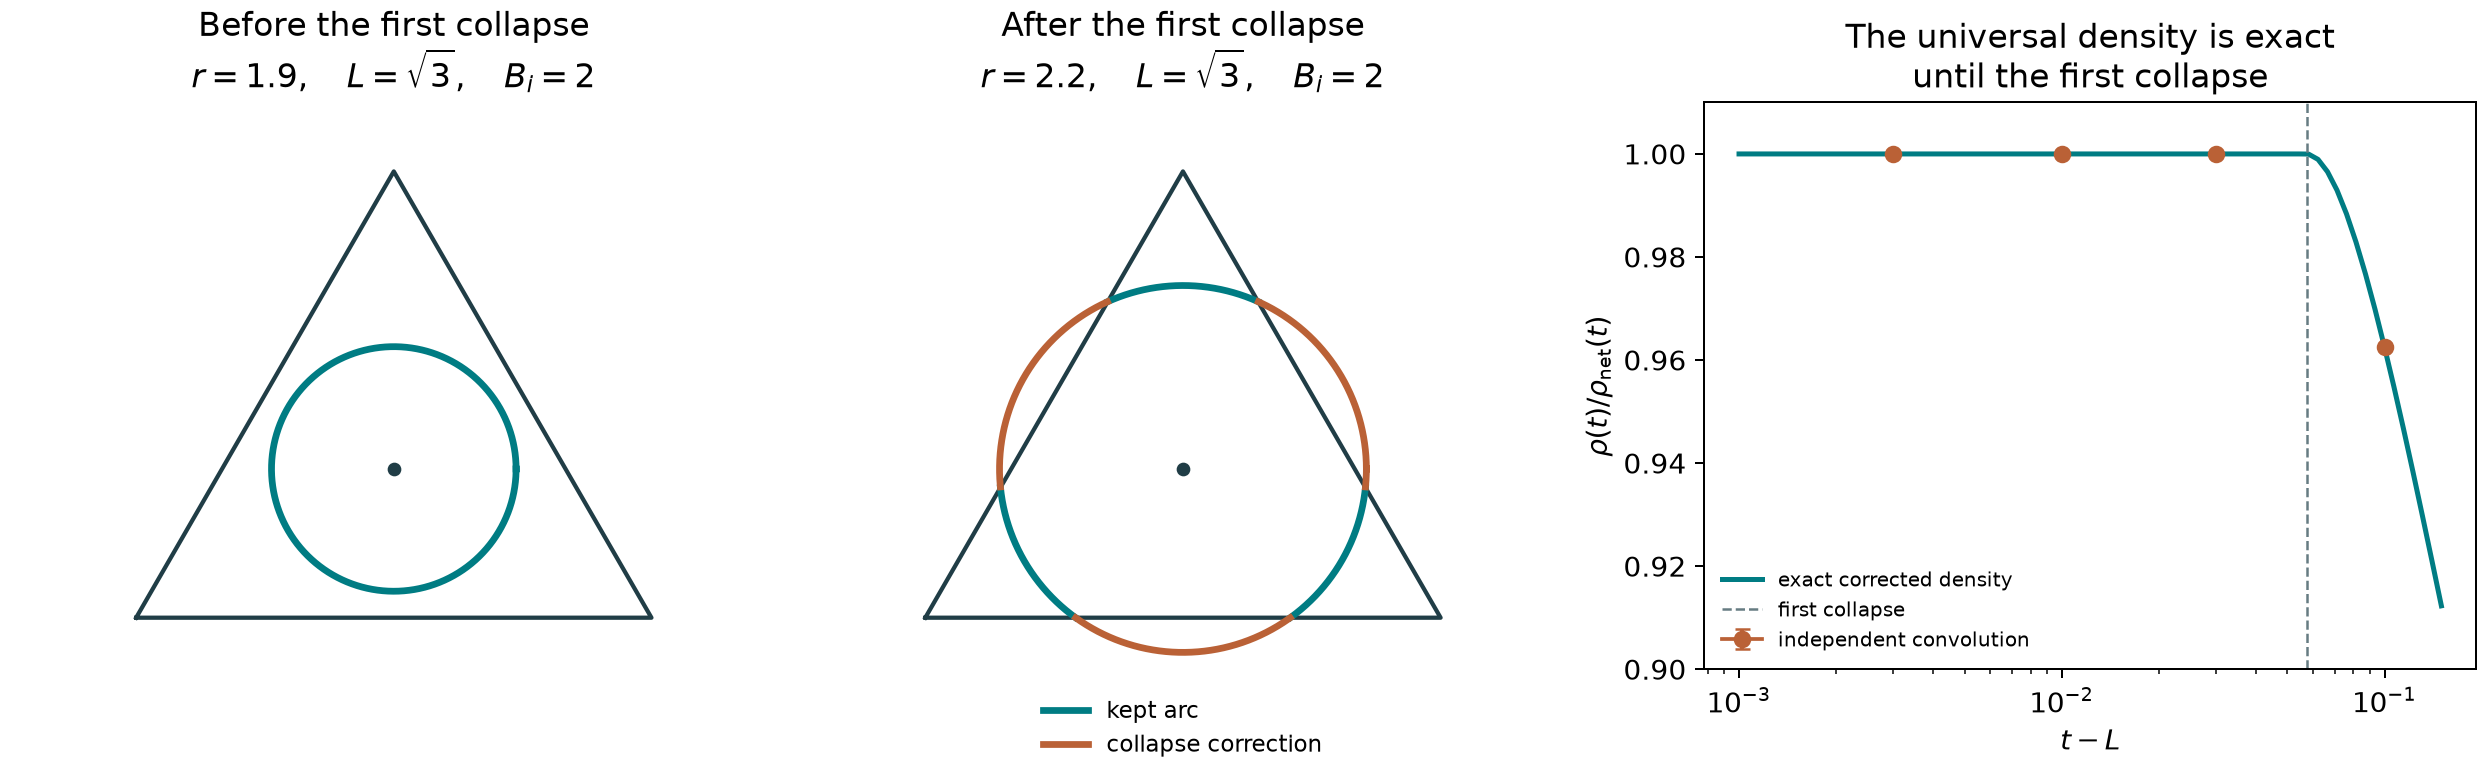
\includegraphics[width=\textwidth]{images/evidence.png}
\end{center}
The script \texttt{scripts/twisted\_net\_trace.py} compares (2) with
independent positive two-dimensional proper-time quadrature in six
triangle shapes at \(\kappa=1/2,1,2,5\). The largest observed relative
discrepancy in 24 checks is \(6.1\cdot10^{-12}\). A near-collapse
triangle has largest angle about \(119.745^\circ\); a control above
\(120^\circ\) is rejected.

An independent Fourier quadrature of the Bloch spectral sum at
\(\kappa=0.7\), cutoff 32 and twist-grid factor 16, gives
\(0.00034489198065699143\), versus
\(0.00034489241045041234\) from (2). The relative discrepancy is
\(1.25\cdot10^{-6}\). Finite coupled-kinetic traces check the simplex
normalization separately. Three unequal-weight cases check (6) by
direct edge-length convolution, with empirical uncertainties.
Raw values are in \texttt{research-data/twisted-nets/results.json}.
Numerical errors are observed, not rigorous continuum certificates.

This is an exact mechanism for theta nets using a family of spectra.
It does not identify one fixed many-body Hamiltonian with all nets,
does not establish a general graph or hyperbolic trace formula, and
does not demonstrate a computational speedup or a Langlands
correspondence. Proper-time methods and geometric descriptions of
Feynman integrals are classical; this note makes no novelty claim.

\begin{thebibliography}{9}
\bibitem{nist} NIST Digital Library of Mathematical Functions,
\href{https://dlmf.nist.gov/10.32}{Section 10.32}.
\bibitem{dd} A.~I.~Davydychev and R.~Delbourgo,
\emph{A geometrical angle on Feynman integrals},
\href{https://arxiv.org/abs/hep-th/9709216}{arXiv:hep-th/9709216}.
\end{thebibliography}
\end{document}
